% License: CC BY-SA
% Authors: See the authors below and see also acknowledgement for authors of some images or research

\documentclass[25pt, margin=0mm, innermargin=25mm, blockverticalspace=25mm, colspace=25mm, subcolspace=8mm]{tikzposter}
\geometry{paperwidth=63in,paperheight=42in}

% to stretch boxes over whole paper with custor paper size
\makeatletter
\setlength{\TP@visibletextwidth}{\textwidth-2\TP@innermargin}
\setlength{\TP@visibletextheight}{\textheight-2\TP@innermargin}
\makeatother

% Fira Sans, GRASS GIS branding sans serif font
\usepackage{FiraSans}
\renewcommand*\oldstylenums[1]{{\firaoldstyle #1}}

% EB Garamond, GRASS GIS branding serif font
% note that EB Garamond does not have bold
\usepackage[cmintegrals,cmbraces]{newtxmath}
\usepackage{ebgaramond-maths}

% might be needed for both font packages
\usepackage[T1]{fontenc}

% uncomment for all sans serif
\renewcommand{\familydefault}{\sfdefault}

\usepackage{setspace}

\usepackage[utf8]{inputenc}
\usepackage{wrapfig}
\usepackage[hidelinks]{hyperref}
\usepackage{alltt}

% For bibliography styling
%% TODO: all names should be abbreviated
\usepackage{natbib}

\definecolor{textcolor}{HTML}{000000}

\definecolor{titleTextColor}{HTML}{000000}
\definecolorpalette{grassColorPalette} {
  \definecolor{colorOne}{HTML}{419041}
  % \definecolor{colorTwo}{HTML}{cccccc}
  \definecolor{colorTwo}{HTML}{dddddd}
  \definecolor{colorThree}{HTML}{F1B52D}
  % \definecolor{colorThree}{HTML}{EFA126}
}

\usetheme{Default}
\usetitlestyle{Empty}
\usecolorstyle[colorPalette=grassColorPalette]{Britain}
\colorlet{backgroundcolor}{white}

\title{
\Huge
\textcolor{titleTextColor}{
\textsf{
% \textbf{
\fontsize{130}{100}\selectfont
\begin{minipage}{\textwidth}
\centering
Software Citation with Fine Granularity:
\\[1cm]
The \textnormal{\textsf{\textit{g.citation}}} Module for \textbf{GRASS}\,{\firalight GIS}
\end{minipage}
% }
}
}
}

\newlength{\grasslogoheight}
\setlength{\grasslogoheight}{0.09\textheight}
\newlength{\instlogoheight}
\setlength{\instlogoheight}{0.33\grasslogoheight}

% \setlength{\blocktitleheight}{0.02\textheight}

% style for institute numbers
\newcommand{\inst}[1]{\hspace{2pt}$^{\mbox{\normalsize#1}}$\hspace{-7pt}}
\newcommand{\instlist}[1]{\hspace{1pt}$^{\mbox{\normalsize#1}}$\hspace{2pt}}

\author{
Vaclav Petras\inst{1}\,*\hspace{-7pt},
Peter Loewe\inst{2},
Markus Neteler\inst{3},
\&
Helena Mitasova\inst{1}
}

\institute{
\large
\instlist{1}Center for Geospatial Analytics, North Carolina State University, USA;
\instlist{2}DIW Berlin Deutsches Institut für Wirtschaftsforschung e.V., Germany;
\instlist{3}mundialis GmbH \& Co. KG, Germany;
*Corresponding author: wenzeslaus@gmail.com, vpetras@ncsu.edu
\\[1.7cm]

\includegraphics[height=3cm]{ncstate}%
\hspace{1cm}%

\includegraphics[height=3cm]{cga}%
\hspace{2.7cm}%

\includegraphics[height=3cm]{diw_berlin}%
\hspace{3cm}%

\includegraphics[height=3.4cm]{mundialis}%
}

% \author{
%
% % Vaclav Petras\inst{1}\,*,
% % Peter Loewe\inst{2},
% % Markus Neteler\inst{3},
% % \&
% % Helena Mitasova\inst{1},
% }
% \institute{
% \large
% % \instlist{1}Center for Geospatial Analytics, North Carolina State University, USA;
% % \instlist{2}DIW Berlin Deutsches Institut für Wirtschaftsforschung e.V., Germany;
% % \instlist{3}mundialis GmbH \& Co. KG, Germany;
% *Corresponding author: wenzeslaus@gmail.com, vpetras@ncsu.edu;
% **Over 10 other members of the core team and numerous other contributors
% \\[1.7cm]
% 
\includegraphics[height=3cm]{ncstate}%
% \hspace{1cm}%
% 
\includegraphics[height=3cm]{cga}%
% \hspace{3cm}%
% 
\includegraphics[height=3.4cm]{mundialis}%
% \hspace{3cm}%
% 
\includegraphics[height=3cm]{diw_berlin}%
% }

\hypersetup
{
    pdfauthor={H. Mitasova, V. Petras, A. Petrasova, M. Neteler},
    pdfsubject={AGU Fall Meeting 2018 Poster},
    pdftitle={Software Citation with Fine Granularity: The g.citation Module for GRASS GIS},
    pdfkeywords={GIS, algorithms, methods, preservation, science, reproducibility}
}

% \usetemplate{1}
% \setinstituteshift{1}

% \setblocktitleheight{2}
% \setblockspacing{1}

\graphicspath{{images/}{logos/}}

\newcommand{\blocktitlewrap}[1]{\textnormal{\textsf{\textsc{\huge#1}}}}
% it is not possible (?) to change block title in the class, using wrapper
% the command introduced using:
%   sed -i 's/\\block{\([^}]*\)}/\\block{\\blocktitlewrap{\1}}/g' main.tex

\newcommand{\CustomBlockFontSize}{\Large}

% bullet point style
\renewcommand{\labelitemi}{\textcolor{gray}{$\bullet$}\hspace{0.5ex}}

% GRASS module
\newcommand{\gmodule}[1]{\href{http://grass.osgeo.org/grass74/manuals/#1.html}{\emph{#1}}}
\newcommand{\gamodule}[1]{\href{http://grass.osgeo.org/grass74/manuals/addons/#1.html}{\emph{#1}}}
\newcommand{\gmodulenolink}[1]{\emph{#1}}

\begin{document}

\node[above left,opacity=0.99,inner sep=0pt,outer sep=6cm] at (bottomleft -| topright)%
  {
\includegraphics[width=0.2\paperwidth]{grass}};

\maketitle[width=0.92\textwidth]

% \maketitle
% \addlogo[north west]{(2,-1)}{9cm}{images/Grass_GIS}
%Please insert your institution logo here
% \addlogo[north east]{(-2,-2.5)}{4cm}{images/logo_FEM_CRI}
% \addlogo[north east]{(-2,-5.5)}{4cm}{images/NC_State_Seal}
% \addlogo[north east]{(-8,-2.5)}{4cm}{images/Logo_cvut}
% \addlogo[north east]{(-8,-6.5)}{4cm}{images/IWMI_logo}
% \addlogo[north east]{(-2,-10.5)}{4cm}{images/logo_ec-jrc}

\begin{columns}

% Session
%
% IN43C: FAIR Data Is Not Enough: Communicating Data Quality and Making Analytical Code FAIR Posters
%
% Regardless of the scientific discipline, a fundamental characteristic of
% science is the exploration of truth, which implies transparency of methods of
% analysis and interpretation as well as understanding imperfections in data to
% arrive at sound conclusions. Fundamental to such understanding is conveying
% accurate and rich information about the observations, analytical source code,
% outputs, and scientific findings.
%
% Source code used in data analysis, like the data themselves, needs to be
% Findable, Accessible, Interoperable and Reusable (FAIR): it also needs to be
% properly versioned, curated and archived to ensure research outcomes can be
% validated.
%
% This session seeks to explore community best practices, challenges, cost,
% benefits, and recommendations for how conveying uncertainty information can be
% made more consistent across multiple Earth science domains and how to manage,
% cite, discover, and share software source code.
%
% Abstract
%
% GRASS GIS (grass.osgeo.org) is a community-driven geospatial software project
% with a record of being used in scientific publications and research projects
% over three decades. Authors of scientific publications, when using and citing
% GRASS GIS, so far opted for citing either the entire software package, citing
% the most recent review publication associated with GRASS GIS, or citing a
% publication associated with a specific module.
%
% GRASS GIS provides over 500 modules, each with a unique functionality and
% purpose, many with associated scientific publications. In addition to these core
% modules in the GRASS GIS distribution there is a growing number of additional
% add-on modules are being developed, often as part of research work. Until now,
% no automated, software-enabled citation mechanism to cite individual GRASS GIS
% modules, or functions in general was provided due to the lack of a reference
% citation standard for GRASS GIS modules defined within the GRASS GIS community.
%
% We present a new GRASS GIS module g.citation with the aim to provide a
% convenient, concise, and standardized way of citing GRASS GIS and its individual
% modules. The current version of g.citation extracts the relevant information
% from a respective manual page of any given GRASS GIS module and turns this
% semi-structured record into a proper citation in a variety of styles and formats
% with the machine-readable Citation File Format (CFF) currently promising most
% efficiency and expressiveness in storing the information and Citation Style
% Language (CSL) used for formatting citations. The module is now in a prototype
% stage and it is available in the GRASS GIS Addons repository. Future directions
% include using standardized format for storing the citation information together
% with the code and incorporating persistent scientific identifiers such as DOI.
% We are now seeking collaborators and feedback from authors of geospatial
% algorithms who want to share their code and be cited at the same time.

%%%%%%%%%%%%%%%%%%%%%%%%%%%%%%%%%%%%%%%%%%%%%%%%%%%%%%%%%%%%%%%%%%%%%
%%%%%%%%%%%%%%%%%%%%%%%%%%%%%%%%%%%%%%%%%%%%%%%%%%%%%%%%%%%%%%%%%%%%%
%%%%%%%%%%%%%%%%%%%%%%%%%%%%%%%%%%%%%%%%%%%%%%%%%%%%%%%%%%%%%%%%%%%%%
%%%%%%%%%%%%%%%%%%%%%%%%%%%%%%%%%%%%%%%%%%%%%%%%%%%%%%%%%%%%%%%%%%%%%
\column{0.25}

%%%%%%%%%%%%%%%%%%%%%%%%%%%%%%%%%%%%%%%%%%%%%%%%%%%%%%%%%%%%%%%%%%%%%%%%%%%%%%%
\block{\blocktitlewrap{GRASS GIS Overview}}{

\CustomBlockFontSize

\begin{itemize}
% Basic Topics
 \item Mature OSGeo Foundation project
 \item Community-driven, user-focused development
 \item 35 years of continuous software development
 \item Long-term releases, stable APIs, and emphasis on science
 \item Single integrated environment for 2D and 3D raster analysis, image processing, vector data analysis, and spatio-temporal data processing
\end{itemize}

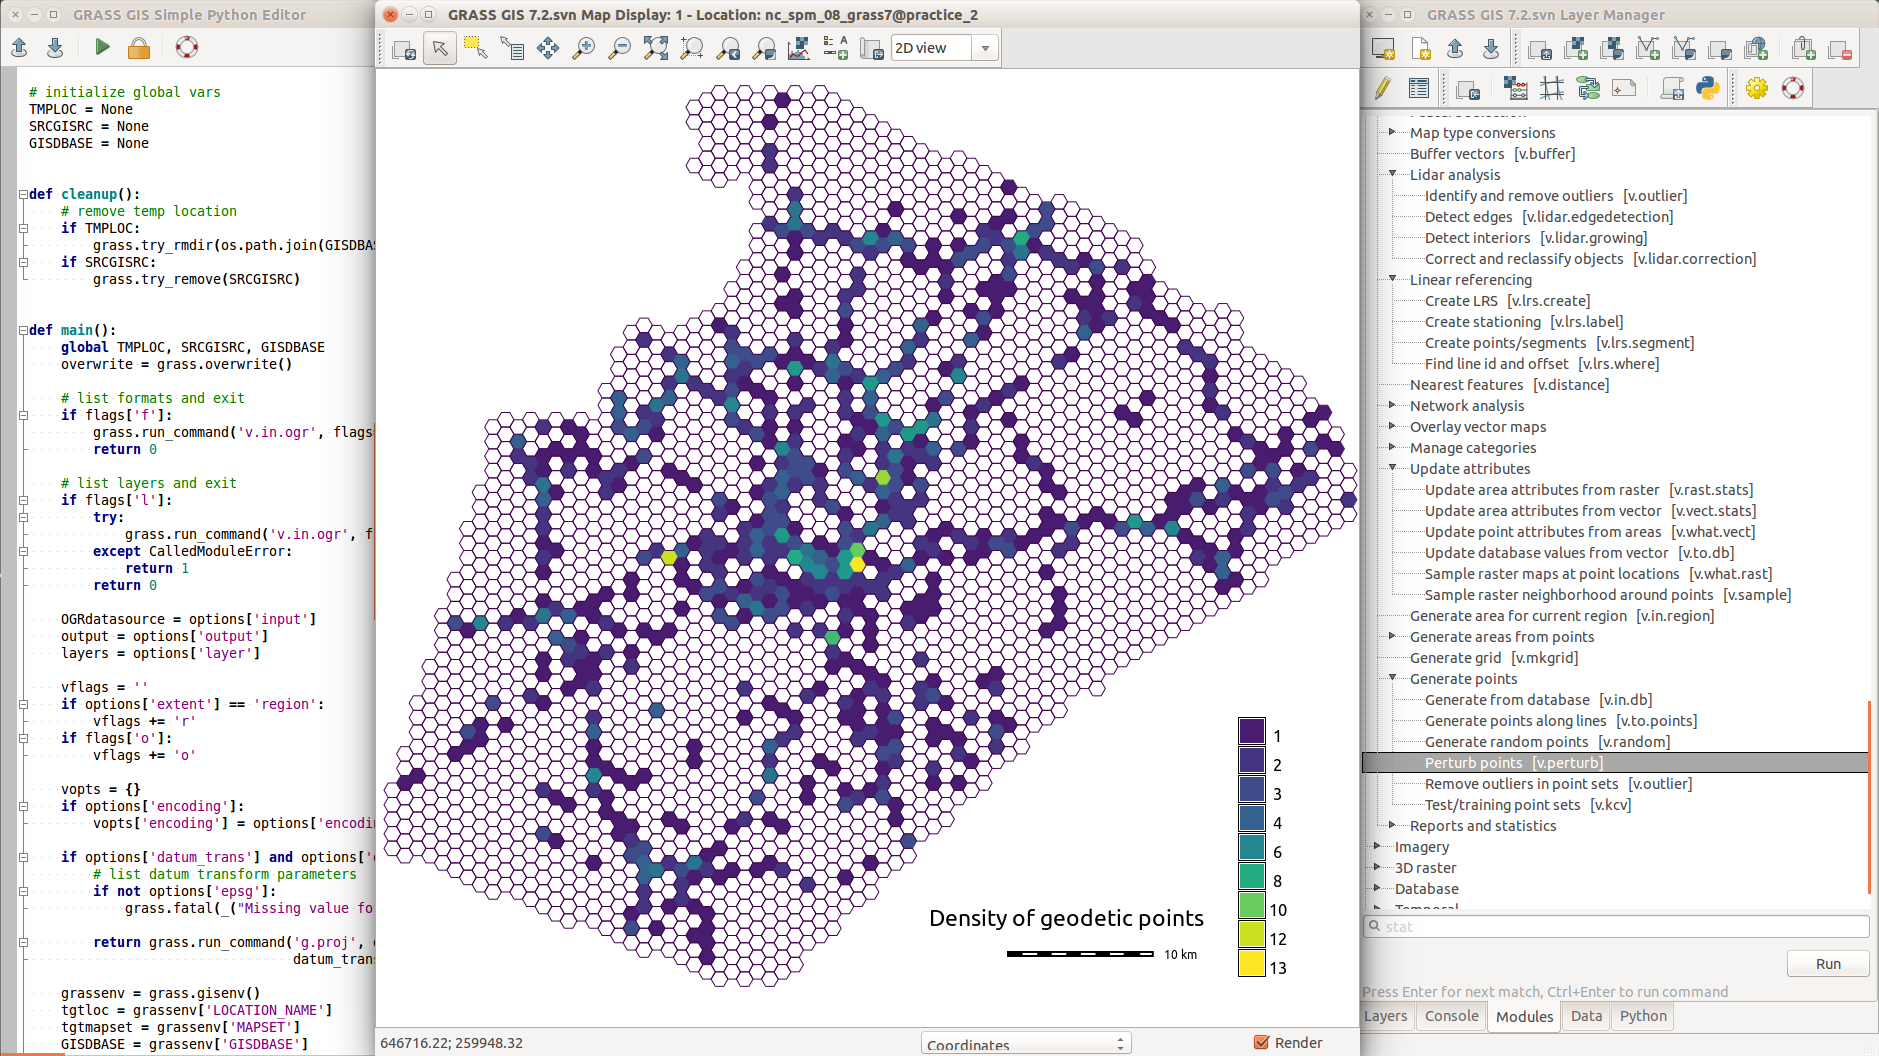
\includegraphics[width=\linewidth]{hexagons_python_editor}

}

%%%%%%%%%%%%%%%%%%%%%%%%%%%%%%%%%%%%%%%%%%%%%%%%%%%%%%%%%%%%%%%%%%%%%%%%%%%%%%%
\block{\blocktitlewrap{Current Approaches}}{

\CustomBlockFontSize

When using GRASS GIS for scientific publication, authors:

\begin{itemize}
 \item cite the entire GRASS GIS software package,
 \item cite a review publication associated with GRASS GIS,
 \item cite a book about GRASS GIS, or
 \item cite a publication associated with a specific module.
\end{itemize}

}


%%%%%%%%%%%%%%%%%%%%%%%%%%%%%%%%%%%%%%%%%%%%%%%%%%%%%%%%%%%%%%%%%%%%%%%%%%%%%%%
\block{\blocktitlewrap{GRASS GIS Documentation}}{

\CustomBlockFontSize

% \vspace*{1.5cm}

\begin{minipage}{\linewidth}
\centering
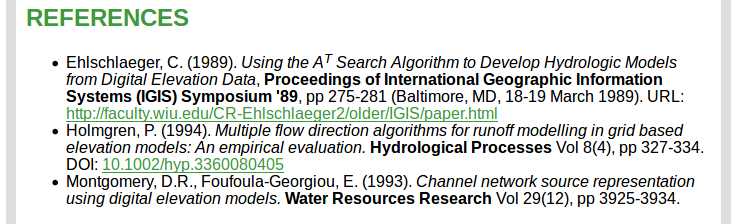
\includegraphics[width=.7\linewidth]{module_references}
\\
% References section contains papers the code is based on, papers published with the code, and papers using the code.
Papers relevant to the code and method in any way
\end{minipage}

\vspace*{1.5cm}

\begin{minipage}{\linewidth}
\centering

\includegraphics[width=.7\linewidth]{module_author}
\\
Authors of code and documentation
\end{minipage}

% \vspace*{1cm}

}


%%%%%%%%%%%%%%%%%%%%%%%%%%%%%%%%%%%%%%%%%%%%%%%%%%%%%%%%%%%%%%%%%%%%%
%%%%%%%%%%%%%%%%%%%%%%%%%%%%%%%%%%%%%%%%%%%%%%%%%%%%%%%%%%%%%%%%%%%%%
%%%%%%%%%%%%%%%%%%%%%%%%%%%%%%%%%%%%%%%%%%%%%%%%%%%%%%%%%%%%%%%%%%%%%
%%%%%%%%%%%%%%%%%%%%%%%%%%%%%%%%%%%%%%%%%%%%%%%%%%%%%%%%%%%%%%%%%%%%%
\column{0.25}


%%%%%%%%%%%%%%%%%%%%%%%%%%%%%%%%%%%%%%%%%%%%%%%%%%%%%%%%%%%%%%%%%%%%%%%%%%%%%%%
\block{\blocktitlewrap{The Challenge}}{

\CustomBlockFontSize

\begin{itemize}
 \item Over 500 core modules and over 300 additional modules
 \item each with a unique functionality and
purpose
 \item many with associated scientific publications.
 \item Until now,
no automated, software-enabled citation mechanism to cite individual GRASS GIS
modules, or functions in general was provided due to the lack of a reference
citation standard for GRASS GIS modules defined within the GRASS GIS community.
 \item no way to cite unless there is a publication
 \item not clear how to identify this publication
 \item publication may not include all current code authors
\end{itemize}

}

% %%%%%%%%%%%%%%%%%%%%%%%%%%%%%%%%%%%%%%%%%%%%%%%%%%%%%%%%%%%%%%%%%%%%%%%%%%%%%%%
% \block{\blocktitlewrap{GRASS GIS Metadata for Modules}}{
%
% \CustomBlockFontSize
%
%
% }

%%%%%%%%%%%%%%%%%%%%%%%%%%%%%%%%%%%%%%%%%%%%%%%%%%%%%%%%%%%%%%%%%%%%%%%%%%%%%%%
\block{\blocktitlewrap{\textnormal{\textsf{\textit{g.citation}}} Module}}{

\CustomBlockFontSize

\vspace*{1.5cm}

\begin{minipage}{\linewidth}
\centering
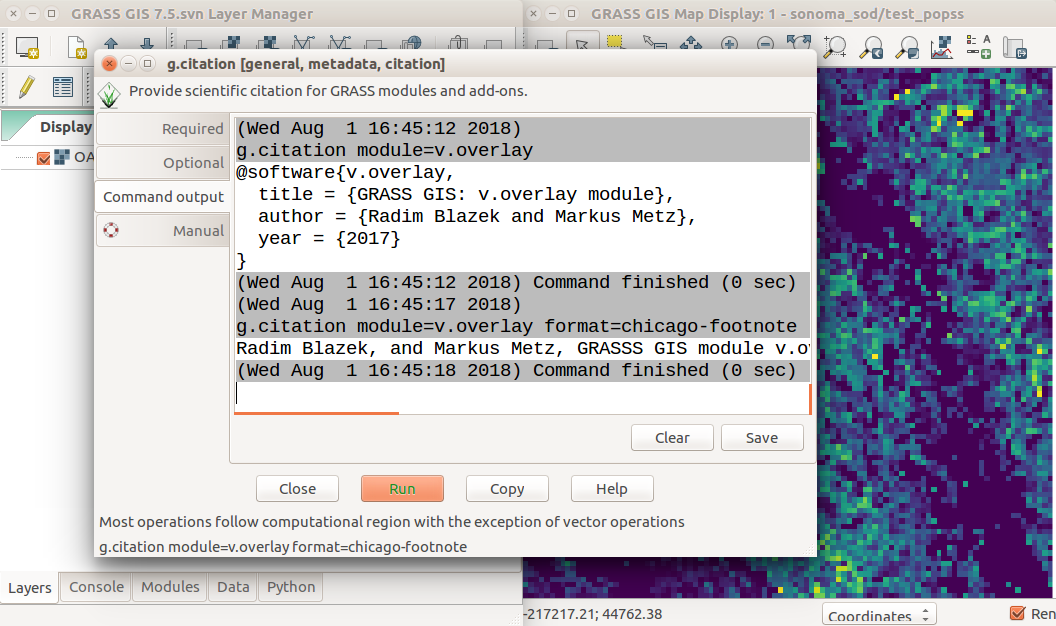
\includegraphics[width=.7\linewidth]{screenshot_bibtex_chicago}
\\
...g.citation GUI...
\end{minipage}

\vspace*{1cm}

}

%%%%%%%%%%%%%%%%%%%%%%%%%%%%%%%%%%%%%%%%%%%%%%%%%%%%%%%%%%%%%%%%%%%%%%%%%%%%%%%
\block{\blocktitlewrap{Citation File Format (CFF)}}{

\CustomBlockFontSize

\begin{itemize}
 \item YAML (YAML Ain’t Markup Language) text file
 \item human- and machine- readable
 \item \texttt{CITATION.cff} file
\end{itemize}

\vspace*{.5cm}

\begin{minipage}{\linewidth}
\centering
\includegraphics[width=.7\linewidth]{code/cff}
\\
...CFF example...
\end{minipage}

\vspace*{1cm}

}

%%%%%%%%%%%%%%%%%%%%%%%%%%%%%%%%%%%%%%%%%%%%%%%%%%%%%%%%%%%%%%%%%%%%%%%%%%%%%%%
\block{\blocktitlewrap{Citation Style Language (CSL)}}{

\CustomBlockFontSize

\begin{itemize}
 \item style language for citations
 \item citeproc-py CSL processor
 \item metadata $\rightarrow$ CSL + citeproc JSON $\rightarrow$ journal citation
\end{itemize}

}

%%%%%%%%%%%%%%%%%%%%%%%%%%%%%%%%%%%%%%%%%%%%%%%%%%%%%%%%%%%%%%%%%%%%%
%%%%%%%%%%%%%%%%%%%%%%%%%%%%%%%%%%%%%%%%%%%%%%%%%%%%%%%%%%%%%%%%%%%%%
%%%%%%%%%%%%%%%%%%%%%%%%%%%%%%%%%%%%%%%%%%%%%%%%%%%%%%%%%%%%%%%%%%%%%
%%%%%%%%%%%%%%%%%%%%%%%%%%%%%%%%%%%%%%%%%%%%%%%%%%%%%%%%%%%%%%%%%%%%%
\column{0.25}

%%%%%%%%%%%%%%%%%%%%%%%%%%%%%%%%%%%%%%%%%%%%%%%%%%%%%%%%%%%%%%%%%%%%%%%%%%%%%%%
\block{\blocktitlewrap{\textnormal{\textsf{\textit{g.citation}}} Example Workflow}}{

\CustomBlockFontSize

\begin{minipage}{\linewidth}
\centering
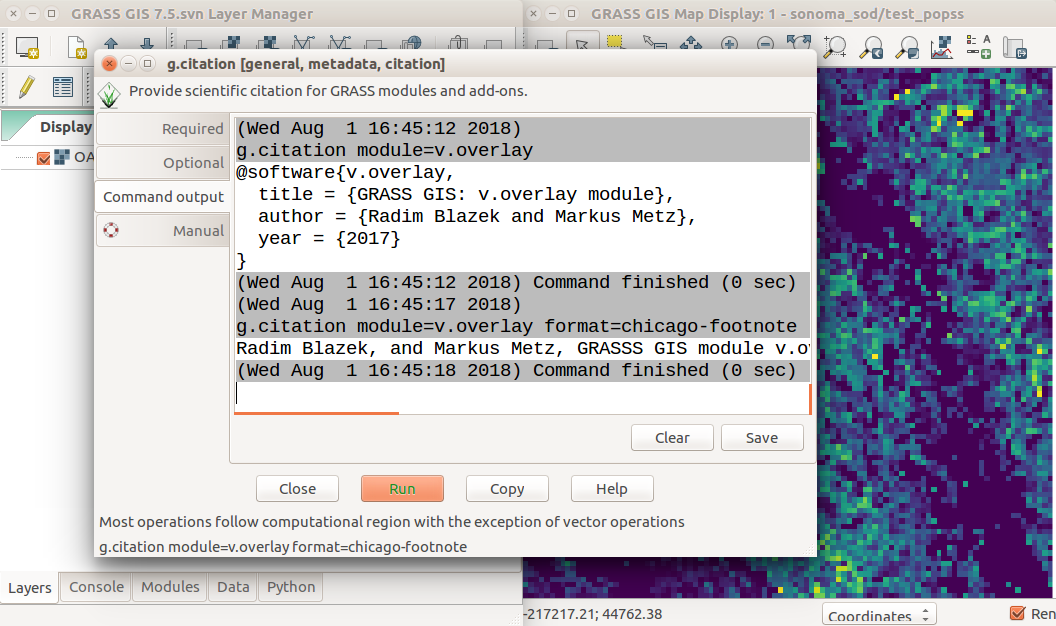
\includegraphics[width=.7\linewidth]{screenshot_bibtex_chicago}
\\
1. Module is used to create XY
\end{minipage}

\vspace*{2ex}

\begin{minipage}{\linewidth}
\centering
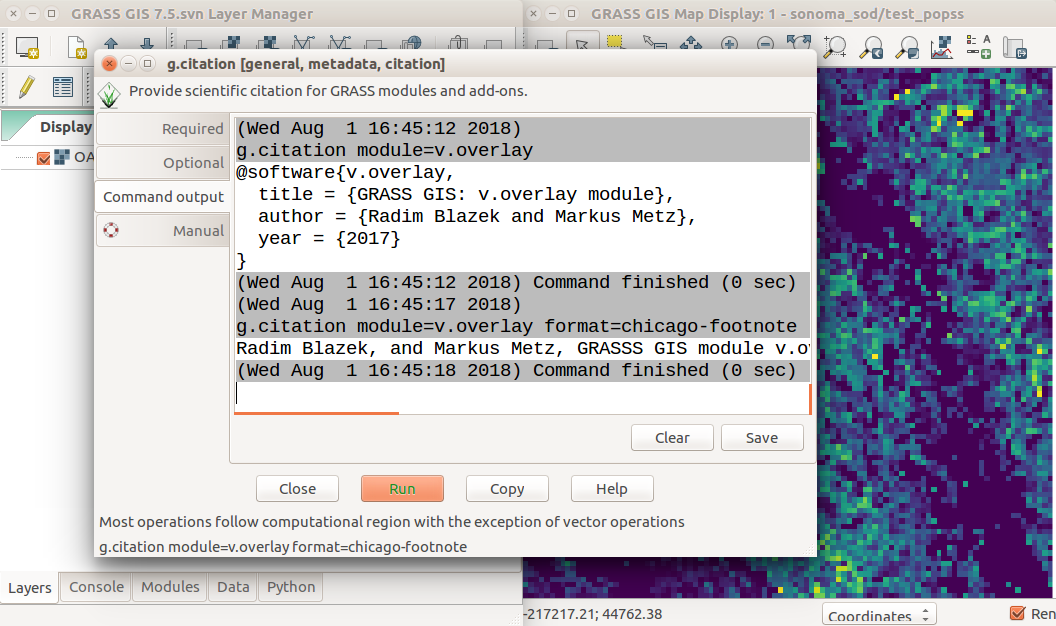
\includegraphics[width=.7\linewidth]{screenshot_bibtex_chicago}
\\
2a. X Citation is created using g.citation
\end{minipage}

\vspace*{2ex}

\begin{minipage}{\linewidth}
\centering
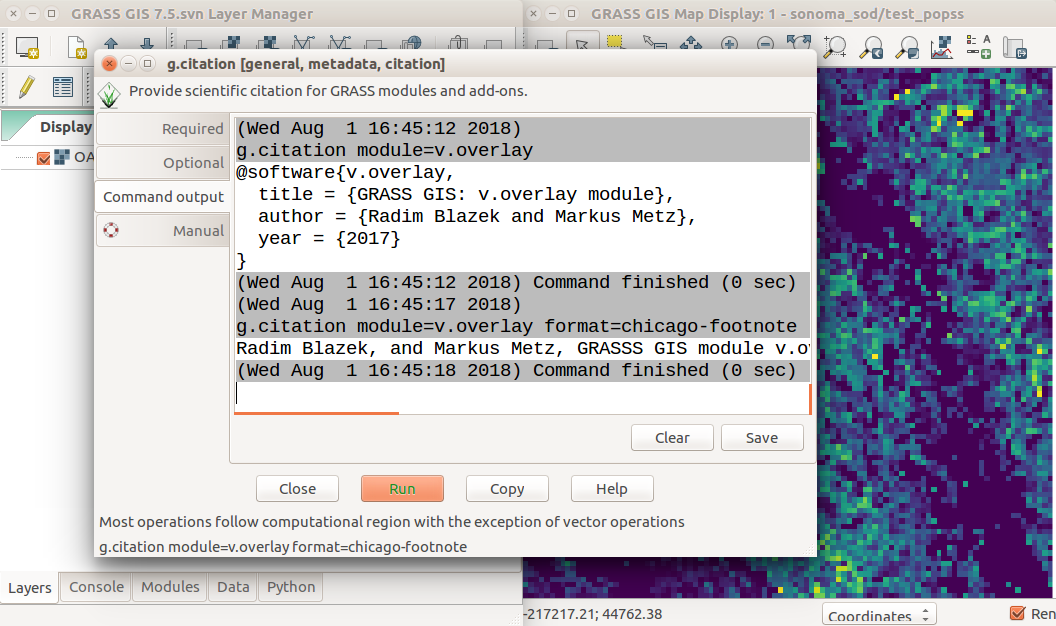
\includegraphics[width=.7\linewidth]{screenshot_bibtex_chicago}
\\
2b. BibTeX Citation is created using g.citation
\end{minipage}

\vspace*{2ex}

\begin{minipage}{\linewidth}
\centering
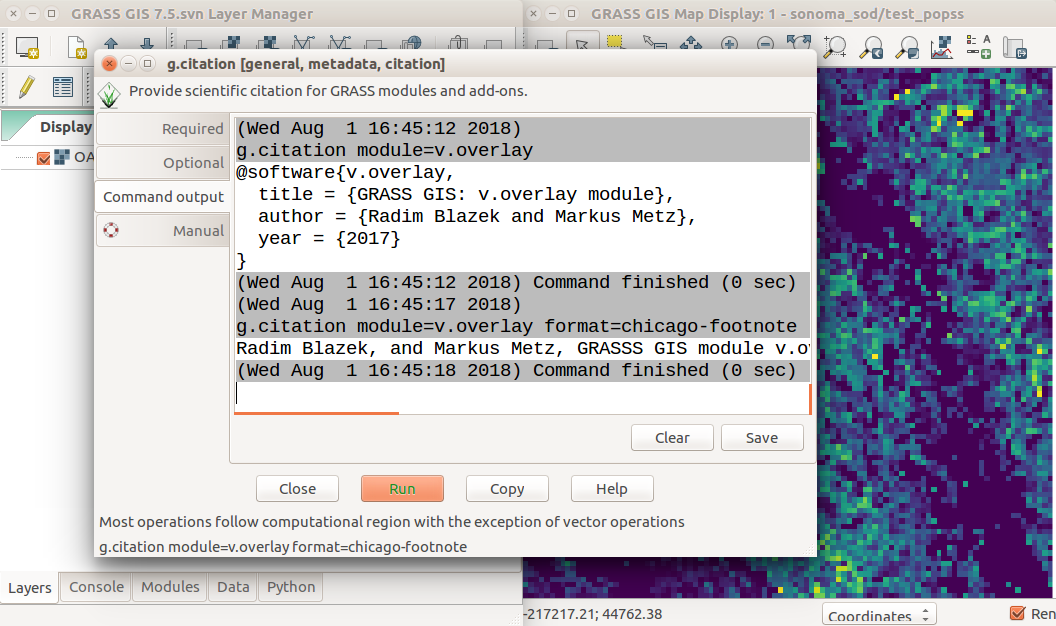
\includegraphics[width=.7\linewidth]{screenshot_bibtex_chicago}
\\
3a. X Citation included in document
\end{minipage}

\vspace*{2ex}

\begin{minipage}{\linewidth}
\centering
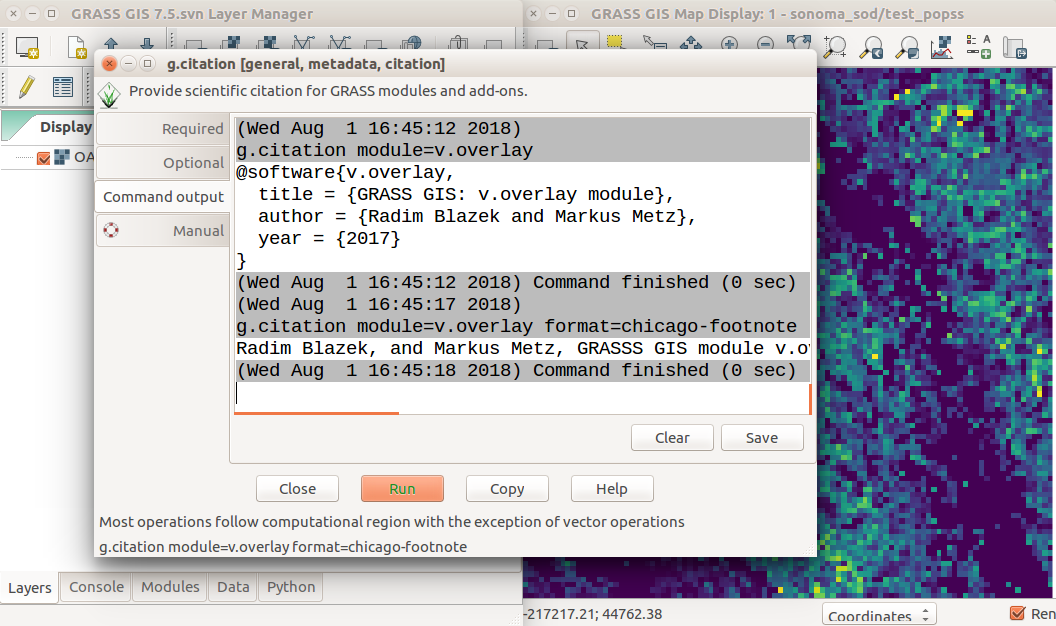
\includegraphics[width=.7\linewidth]{screenshot_bibtex_chicago}
\\
3b. BibTeX citation is pasted to Zotero
\end{minipage}

\vspace*{2ex}

\begin{minipage}{\linewidth}
\centering
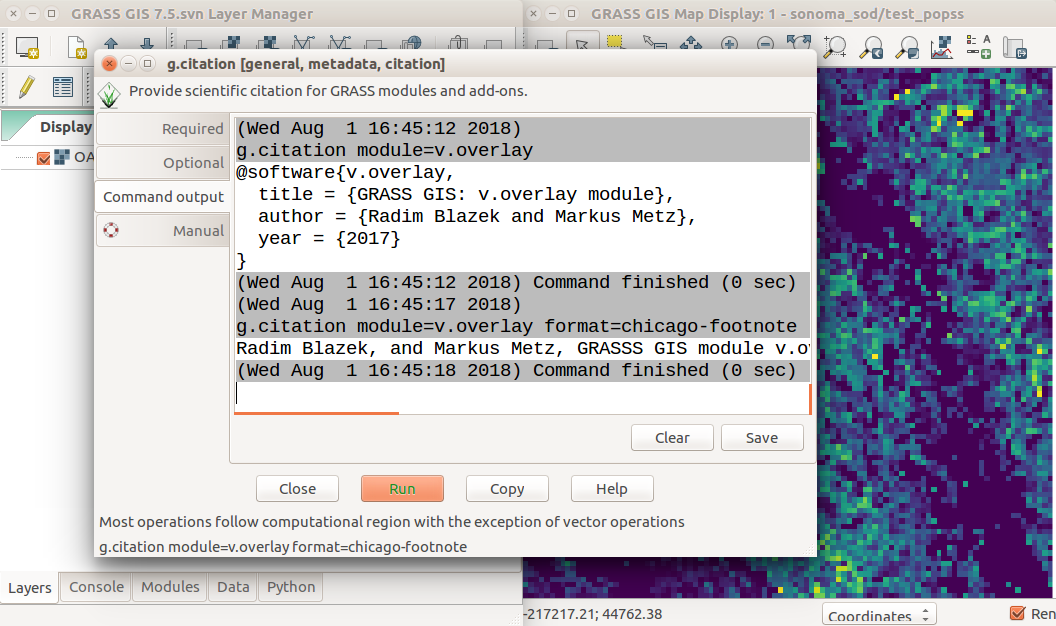
\includegraphics[width=.7\linewidth]{screenshot_bibtex_chicago}
\\
3c. BibTeX citation is pasted to Overleaf
\end{minipage}

}

%%%%%%%%%%%%%%%%%%%%%%%%%%%%%%%%%%%%%%%%%%%%%%%%%%%%%%%%%%%%%%%%%%%%%%%%%%%%%%%
\block{\blocktitlewrap{Discussion and Future Work}}{

\CustomBlockFontSize


}


%%%%%%%%%%%%%%%%%%%%%%%%%%%%%%%%%%%%%%%%%%%%%%%%%%%%%%%%%%%%%%%%%%%%%%%%%%%%%%%%
\block{\blocktitlewrap{References}}{

\vspace{-0.2cm}

% \newcommand{\blocksectiontitle}[1]{\subsubsection*{\textcolor{gray}{\textsf{#1}}}}
\newcommand{\blocksectiontitle}[1]{\textbf{#1}}

%\blocksectiontitle{References}
\begingroup
\renewcommand{\section}[2]{}%
\bibliographystyle{apalike}
\setstretch{0.5}
\scriptsize
\bibliography{poster}
\endgroup

}

%%%%%%%%%%%%%%%%%%%%%%%%%%%%%%%%%%%%%%%%%%%%%%%%%%%%%%%%%%%%%%%%%%%%%
%%%%%%%%%%%%%%%%%%%%%%%%%%%%%%%%%%%%%%%%%%%%%%%%%%%%%%%%%%%%%%%%%%%%%
%%%%%%%%%%%%%%%%%%%%%%%%%%%%%%%%%%%%%%%%%%%%%%%%%%%%%%%%%%%%%%%%%%%%%
%%%%%%%%%%%%%%%%%%%%%%%%%%%%%%%%%%%%%%%%%%%%%%%%%%%%%%%%%%%%%%%%%%%%%
\column{0.25}


%%%%%%%%%%%%%%%%%%%%%%%%%%%%%%%%%%%%%%%%%%%%%%%%%%%%%%%%%%%%%%%%%%%%%%%%%%%%%%%
\block{\blocktitlewrap{GRASS GIS as a Scientific Code Repository}}{

\CustomBlockFontSize

\begin{itemize}
 \item Innovations are preserved \citep{chemin2015grass}
 \item Code is further developed \citep{petras_how_2017}
 \item Tools used by other scientists \citep{petras2018grass} [AGU 2018]
\end{itemize}

}

%%%%%%%%%%%%%%%%%%%%%%%%%%%%%%%%%%%%%%%%%%%%%%%%%%%%%%%%%%%%%%%%%%%%%%%%%%%%%%%
\block{\blocktitlewrap{Availability}}{

\CustomBlockFontSize

\begin{itemize}
 \item \href{https://grass.osgeo.org}{grass.osgeo.org}
 \item g.citation part of GRASS GIS Addons repository
 \item Code under GNU GPL >=v2 (SPDX: GPL-2.0-or-later)
 \item Poster under CC Attribution-ShareAlike 4.0 International
\end{itemize}

}

\end{columns}

\end{document}
